\documentclass[11pt]{article}
\usepackage[margin=1in]{geometry}
\usepackage{amsmath}
\usepackage{amssymb}
\usepackage{tikz}

\setlength{\parindent}{0pt}

\begin{document}

\textbf{Question 8.2}
\bigskip

The probability distribution of a less risky expected return is more peaked than that of a riskier return. What shape would the probability distribution be for (a) completely certain returns and (b) completely uncertain returns?

\bigskip
\textbf{Answer}

\begin{enumerate}
  \item[a.] For completely certain returns, the distribution collapses to a single vertical spike at the certain value. All probability mass is concentrated on one outcome, so the standard deviation is zero.
  \item[b.] For completely uncertain returns, the distribution is perfectly flat (uniform) across the entire range of possible outcomes. No outcome is more likely than any other, and dispersion is at its maximum.
\end{enumerate}

\bigskip
\bigskip

\textbf{Question 8.22}
\bigskip

Bartman Industries's and Reynolds Inc.'s stock prices and dividends, along with the Winslow 5000 Index (adjusted to include dividends), are given for 2012--2017. Calculate annual returns, average returns, standard deviations, coefficients of variation, and Sharpe ratios; then construct a scatter diagram of Bartman's and Reynolds's returns against the Winslow 5000.

\bigskip
\textbf{Answer}

\begin{enumerate}
  \item[a.] Annual return for stocks: $r_t = (P_t + D_t - P_{t-1}) / P_{t-1}$. For the Winslow index (already includes dividends): $r_t = (I_t - I_{t-1}) / I_{t-1}$. The 2012 return cannot be computed (no 2011 data), so five returns (2013--2017) are used.

    \medskip

    \textit{Bartman:}
    \begin{align*}
      r_{2013} &= (11.37+0.90-7.62)/7.62 = 61.02\%\\
      r_{2014} &= (10.75+0.95-11.37)/11.37 = 2.90\%\\
      r_{2015} &= (16.50+1.00-10.75)/10.75 = 62.79\%\\
      r_{2016} &= (14.75+1.06-16.50)/16.50 = -4.18\%\\
      r_{2017} &= (17.25+1.15-14.75)/14.75 = 24.75\%
    \end{align*}
    \[
      \boxed{\bar{r}_{\text{Bartman}} \approx 29.46\%}
    \]

    \textit{Reynolds:}
    \begin{align*}
      r_{2013} &= (60.00+2.25-55.75)/55.75 = 11.66\%\\
      r_{2014} &= (57.25+2.50-60.00)/60.00 = -0.42\%\\
      r_{2015} &= (48.75+2.75-57.25)/57.25 = -10.04\%\\
      r_{2016} &= (52.30+2.90-48.75)/48.75 = 13.23\%\\
      r_{2017} &= (48.75+3.00-52.30)/52.30 = -1.05\%
    \end{align*}
    \[
      \boxed{\bar{r}_{\text{Reynolds}} \approx 2.68\%}
    \]

    \textit{Winslow 5000:}
    \begin{align*}
      r_{2013} &= (5{,}602.28-4{,}705.97)/4{,}705.97 = 19.05\%\\
      r_{2014} &= (6{,}434.03-5{,}602.28)/5{,}602.28 = 14.85\%\\
      r_{2015} &= (8{,}679.98-6{,}434.03)/6{,}434.03 = 34.91\%\\
      r_{2016} &= (8{,}785.70-8{,}679.98)/8{,}679.98 = 1.22\%\\
      r_{2017} &= (11{,}663.98-8{,}785.70)/8{,}785.70 = 32.76\%
    \end{align*}
    \[
      \boxed{\bar{r}_{\text{Winslow}} \approx 20.56\%}
    \]

  \item[b.] Sample standard deviation: $\sigma = \sqrt{\frac{1}{n-1}\sum_{i=1}^{n}(r_i-\bar{r})^2}$ with $n=5$:
    \[
      \boxed{\sigma_{\text{Bartman}} \approx 31.49\%, \quad \sigma_{\text{Reynolds}} \approx 9.71\%, \quad \sigma_{\text{Winslow}} \approx 13.82\%}
    \]

  \item[c.] Coefficient of variation $\text{CV} = \sigma/\bar{r}$:
    \begin{align*}
      \text{CV}_{\text{Bartman}}  &= 31.49/29.46 \approx 1.069\\
      \text{CV}_{\text{Reynolds}} &= 9.71/2.68  \approx 3.628\\
      \text{CV}_{\text{Winslow}}  &= 13.82/20.56 \approx 0.672
    \end{align*}
    Per unit of return earned, Reynolds is the riskiest, the Winslow Index is the least risky, and Bartman is in between.

  \item[d.] Sharpe ratio $S = (\bar{r}-r_f)/\sigma$ with $r_f = 3\%$:
    \begin{align*}
      S_{\text{Bartman}}  &= (29.46-3)/31.49 \approx 0.840\\
      S_{\text{Reynolds}} &= (2.68-3)/9.71  \approx -0.033\\
      S_{\text{Winslow}}  &= (20.56-3)/13.82 \approx 1.270
    \end{align*}
    The Winslow Index delivers the best risk-adjusted return; Reynolds's negative Sharpe ratio means it underperformed the risk-free asset on a risk-adjusted basis over this period.

  \item[e.] Scatter diagram of Bartman's and Reynolds's returns (vertical axis) against the Winslow 5000's returns (horizontal axis):

    \begin{center}
    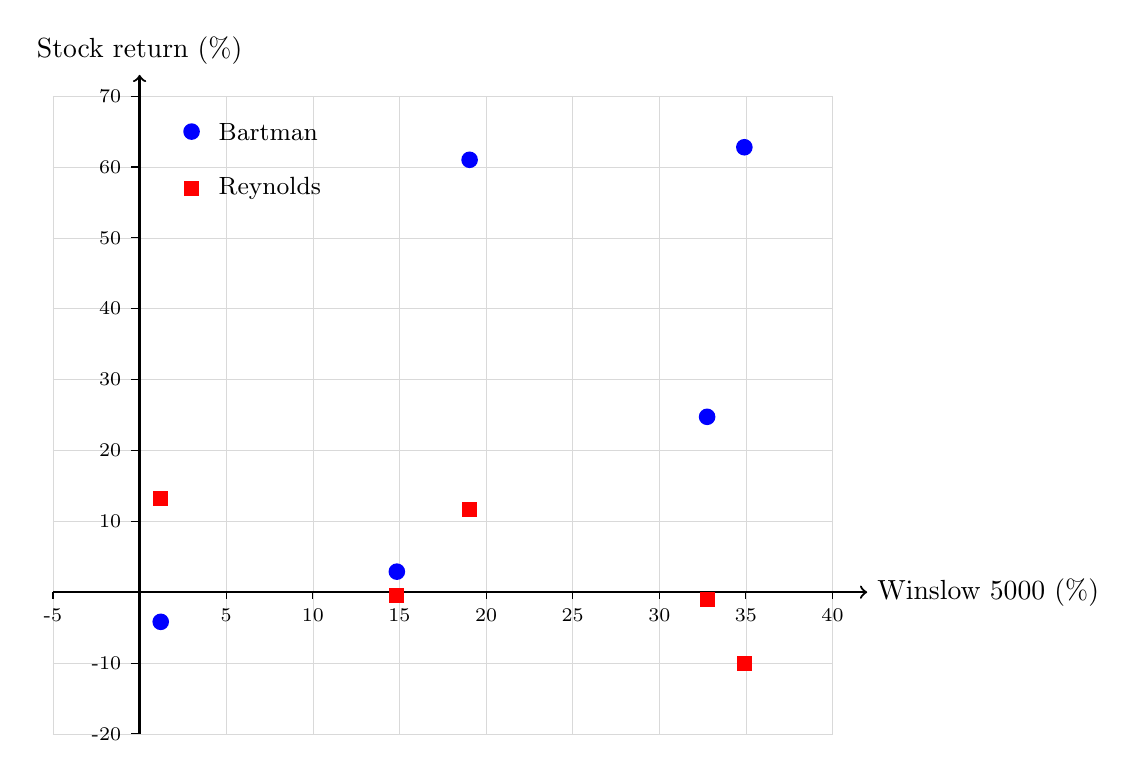
\begin{tikzpicture}[x=0.22cm, y=0.09cm]
      % gridlines
      \draw[very thin, gray!30] (-5,-20) grid[xstep=5, ystep=10] (40,70);
      % axes
      \draw[->, thick] (-5,0) -- (42,0) node[right] {Winslow 5000 (\%)};
      \draw[->, thick] (0,-20) -- (0,73) node[above] {Stock return (\%)};
      % x ticks
      \foreach \x in {-5,5,10,15,20,25,30,35,40}
        \draw (\x,0) -- (\x,-1) node[below, font=\scriptsize] {\x};
      % y ticks
      \foreach \y in {-20,-10,10,20,30,40,50,60,70}
        \draw (0,\y) -- (-0.5,\y) node[left, font=\scriptsize] {\y};
      % Bartman points (blue circles)
      \foreach \p in {(19.05,61.02),(14.85,2.90),(34.91,62.79),(1.22,-4.18),(32.76,24.75)}
        \fill[blue] \p circle (3pt);
      % Reynolds points (red squares)
      \foreach \p in {(19.05,11.66),(14.85,-0.42),(34.91,-10.04),(1.22,13.23),(32.76,-1.05)}
        \draw[red, fill=red] \p +(-2.5pt,-2.5pt) rectangle +(2.5pt,2.5pt);
      % Legend
      \fill[blue] (3,65) circle (3pt);
      \node[right, font=\small] at (4,65) {Bartman};
      \draw[red, fill=red] (3,57) +(-2.5pt,-2.5pt) rectangle +(2.5pt,2.5pt);
      \node[right, font=\small] at (4,57) {Reynolds};
    \end{tikzpicture}
    \end{center}

    Bartman's points slope upward with the index, indicating a high beta and strong positive co-movement with the market. Reynolds's points are roughly flat or slope downward, suggesting a low or even slightly negative beta.
\end{enumerate}

\end{document}
